\section{The complete small spectrum}\label{sec:spectrum}

Let $\Delta_{\tau,U}=D_U^*D_U$ act on trace-free
$h_0$-Hermitian endomorphisms over $C_\tau$. We use the
unnormalized area norm and the energy
\[
 \mathcal Q_{\tau,U}(s)=\int_{C_\tau}|D_Us|^2\,dA_\tau.
\]
Its eigenvalues $\lambda_0\le\lambda_1\le\cdots$ include
the kernel. With the HYM convention in
Section~\ref{sec:actual-flow}, this is the positive
linearization at $h_0$.

\begin{theorem}\label{thm:spectrum}
For each fixed $r\ge2$ there are $\gamma>0$ and a
function $\epsilon(\tau)\to0$ as $L_*\to\infty$ such that,
uniformly for $U\in\SU(r)^6$ and all positive length ratios,
\begin{equation}\label{eq:relative-spectrum}
 (1-\epsilon(\tau))\nu_k\le\lambda_k
 \le(1+\epsilon(\tau))\nu_k\quad(0\le k<m),
 \qquad \lambda_m\ge\gamma .
\end{equation}
For sufficiently small parameters exactly $m$ eigenvalues
lie below a fixed positive threshold. The actual kernel
is the space of compatible tuples in
\eqref{eq:finite-forms}.
\end{theorem}

The multiplicative error in \eqref{eq:relative-spectrum}
remains meaningful when $\nu_k/w_*$ tends to zero at an
arbitrary rate. Its proof uses the section energy to
control every boundary error. An additive $o(w_*)$ bound
would not imply this assertion.

\subsection{Trial sections}
Fix a small radius $a$ independent of all parameters.
The annulus $|\tau_e|/a<|u_e|<a$ has logarithmic length
$\ell_e=L_e+2\log a$. In its flat node frame, join
$X_i$ to $\Ad(U_{ij})X_j$ by affine interpolation in
$\log|u_e|$ and keep the section constant on each
component exterior. The resulting map $J_a:\cV\to H^1$
is continuous across boundary circles; derivative
jumps are allowed in the form domain. Conformal
invariance of the two-dimensional Dirichlet energy gives
the exact identity
\begin{equation}\label{eq:trial-energy}
 \mathcal Q_{\tau,U}(J_aX)
 =\sum_e\frac{2\pi}{\ell_e}
       \|X_i-\Ad(U_{ij})X_j\|^2.
\end{equation}
For fixed $a$ and large $L_*$,
$1\le L_e/\ell_e\le1+C_a/L_*$. By
Lemma~\ref{lem:ambient}, unitarity and smooth exterior
convergence,
\begin{equation}\label{eq:trial-mass}
 \big|\|J_aX\|_{L^2}^2-M(X)\big|
 \le\big(Ca^2+o_a(\tau)\big)M(X),
\end{equation}
where $o_a(\tau)\to0$ for fixed $a$, uniformly in the
unitary parameters. Min--max proves the relative upper
bound with these errors, and gives
$\lambda_{m-1}\le Cw_*$.

\subsection{A weighted lower estimate}
For an arbitrary $H^1$ section $s$ let $b_i(s)$ be its
average, in the flat component frame, over the component
exterior truncated at radius $a/2$. Let $c_{ie}(s)$ be
its angular mean on the circle of radius $a$ at an
incidence. Fixed-domain Poincar\'e and trace inequalities
give
\begin{equation}\label{eq:boundary-mean}
 \|c_{ie}(s)-b_i(s)\|
 \le C_a\mathcal Q_{\tau,U}(s)^{1/2}.
\end{equation}
The circle lies in the interior of the chosen truncated
domain. Thus only uniformly smooth fixed collars are
used in this estimate.

Angular averaging and Cauchy--Schwarz on each node
annulus imply
\[
 \sum_e\widetilde w_e
 \|c_{ie}-\Ad(U_{ij})c_{je}\|^2
 \le\mathcal Q_{\tau,U}(s),
 \qquad \widetilde w_e=2\pi/\ell_e.
\]
Apply the triangle inequality in the direct sum of the
edge spaces weighted by $\sqrt{\widetilde w_e}$.
Equation~\eqref{eq:boundary-mean}, the fixed number of
incidences and $\widetilde w_e\le Cw_*$ give
\[
 \left(\sum_e\widetilde w_e
 \|b_i-\Ad(U_{ij})b_j\|^2\right)^{1/2}
 \le(1+C_a\sqrt{w_*})\mathcal Q_{\tau,U}(s)^{1/2}.
\]
Since $w_e\le\widetilde w_e$, we have proved
\begin{equation}\label{eq:lower-energy}
 \mathcal Q_{\tau,U}(s)\ge
 (1+C_a\sqrt{w_*})^{-2}Q_{\tau,U}(b(s)).
\end{equation}
There is no reciprocal of the smallest edge weight in
this estimate.

\subsection{Mass on the annuli}
We include the estimate which excludes additional
small modes supported on the shrinking regions.

\begin{lemma}\label{lem:zero-boundary}
Let $w$ be a vector-valued $H^1$ function on a node
annulus with zero boundary values at $|u_e|=a$ and
$|v_e|=a$. Then
\[
 \|w\|_{L^2}^2\le Ca^2\int|dw|^2\,dA_\tau,
\]
with $C$ independent of the annular modulus and all
small parameters.
\end{lemma}
\begin{proof}
First use the induced Euclidean metric on the complex
curve in $\CC^2$ and put $f=|u_e|^2+|v_e|^2$.
Its coordinate functions are harmonic, so
$\Delta_+ f=4$ for the divergence-form
operator $\Delta_+=\operatorname{div}\nabla$,
the negative of our nonnegative Laplacian.
Also $|\nabla f|\le Ca$ on the annulus. Integration by
parts, with zero boundary trace, yields
\[
 4\int|w|^2
 =-2\int\langle w,dw\rangle\cdot\nabla f
 \le Ca\|w\|_{L^2}\|dw\|_{L^2}.
\]
Squaring proves the estimate. The same argument applies
to each real coordinate of $w$. Uniform comparison of
areas in Lemma~\ref{lem:ambient} and conformal invariance
of the Dirichlet energy transfer it to the actual metric.
\end{proof}

\begin{lemma}\label{lem:low-mass}
If $s$ belongs to the span of at most $m+1$
orthonormal eigensections with eigenvalues at most
$\Lambda\le1$, then
\begin{equation}\label{eq:low-mass}
 \big|M(b(s))-\|s\|_{L^2}^2\big|
 \le\big(Ca^2+C_a\sqrt{\Lambda}+o_a(\tau)\big)
                 \|s\|_{L^2}^2.
\end{equation}
All constants are uniform in $U$ and in the node-length
ratios.
\end{lemma}
\begin{proof}
Start with a normalized eigensection of eigenvalue
$\lambda\le1$. On a fixed component exterior,
Poincar\'e gives $\|s-b_i\|_{L^2}\le C_a\sqrt\lambda$.
In the flat frame the equation is the scalar
eigenfunction equation in each real coordinate.
Interior $W^{2,2}$ estimates on slightly smaller
fixed collars, followed by the two-dimensional
embedding into $C^0$, give the same order on each
boundary circle. The averages themselves are uniformly
bounded by Cauchy--Schwarz.

On a node annulus write $s=h+w$, where $h$ is the
coordinatewise harmonic extension of its boundary
values and $w$ has zero boundary trace. The maximum
principle bounds $h$ by the boundary supremum, and
the annular area is $O(a^2)$. Orthogonality in
Dirichlet energy gives $E(w)\le E(s)\le\lambda$;
Lemma~\ref{lem:zero-boundary} bounds its mass.
Combining the component and annular estimates yields
\eqref{eq:low-mass} for one eigenfunction. The difference
between the radii $a/2$ used for averaging and $a$
used to partition the surface is covered by the same
component Poincar\'e estimate.

For a unit linear combination of at most $m+1$
orthonormal eigensections, sum the boundary and
exterior estimates and use Cauchy--Schwarz in the
finite coefficient space. Its energy is at most
$\Lambda$. The preceding harmonic-extension argument
then applies without change, with a constant depending
on $m$.
\end{proof}

\begin{proof}[Proof of Theorem~\ref{thm:spectrum}]
If $\lambda_m$ tended to zero along any sequence with
$L_*\to\infty$, choose $a$ small and then use
Lemma~\ref{lem:low-mass} on its first $m+1$
eigensections. Averaging would be injective from an
$(m+1)$-dimensional space to $\cV$, a contradiction.
Thus $\lambda_m\ge\gamma>0$ uniformly. The upper
bound $\lambda_{m-1}\le Cw_*\to0$ identifies precisely
the asserted cluster.

On the span of the first $k+1$ eigensections, $k<m$,
take $\Lambda=Cw_*$. Averaging is injective and
almost isometric. Finite min--max supplies a nonzero
$s$ in that span for which
$Q_{\tau,U}(b(s))\ge\nu_kM(b(s))$. Therefore
\[
 \lambda_k\ge
 \frac{\mathcal Q_{\tau,U}(s)}{\|s\|_{L^2}^2}
 \ge(1+C_a\sqrt{w_*})^{-2}
       \big(1-Ca^2-C_a\sqrt{w_*}-o_a(\tau)\big)\nu_k.
\]
Together with \eqref{eq:trial-energy}--\eqref{eq:trial-mass}
this proves the relative comparison: first choose $a$
for a prescribed error and then take all parameters
sufficiently small. This order gives a single uniform
error modulus tending to zero. No division by $\nu_k$
or by a smallest weight has occurred.

Finally zero energy means that a section is parallel.
It is constant in every flat patch, and its values
obey the edge compatibility relations. Conversely each
compatible tuple extends to such a section. This
proves the exact kernel assertion even when its
dimension changes.
\end{proof}

\begin{corollary}\label{cor:complement}
Let $\Pi_{\tau,U}$ project orthogonally onto the first
$m$ eigensections. On its orthogonal complement,
\[
 \|\Delta_{\tau,U}^{-1}\|_{L^2\to L^2}\le\gamma^{-1},
 \qquad
 \|e^{-s\Delta_{\tau,U}}(1-\Pi_{\tau,U})\|_{L^2\to L^2}
 \le e^{-\gamma s}.
\]
For $z\notin[\gamma,\infty)$ the complementary resolvent
has norm at most $\operatorname{dist}(z,[\gamma,\infty))^{-1}$.
\end{corollary}
\begin{proof}
These are the spectral-calculus bounds for the
nonnegative self-adjoint operator on that subspace.
\end{proof}

These are $L^2$ estimates. They do not assert a uniform
global Schauder or Sobolev estimate on the degenerating
surface.

\subsection{A compact example with three weak scales}
Use the rank-two transports in Example~\ref{ex:noncommuting}
and the Fubini--Study normalization $A_i=1$. For $h>0$ put
\[
 w_{01}=w_{02}=w_{03}=h,\qquad
 w_{12}=h^2,\quad w_{23}=h^3,\quad w_{13}=h^4,
 \qquad \tau_e(h)=e^{-2\pi/w_e(h)}.
\]
This is a real path in the complex family of
Proposition~\ref{prop:compact-family}; it is not claimed
to extend as a holomorphic disc at $h=0$.
Every sufficiently small positive $h$ gives a stable bundle on a smooth
compact genus-three curve.

\begin{figure}[htbp]
 \centering
 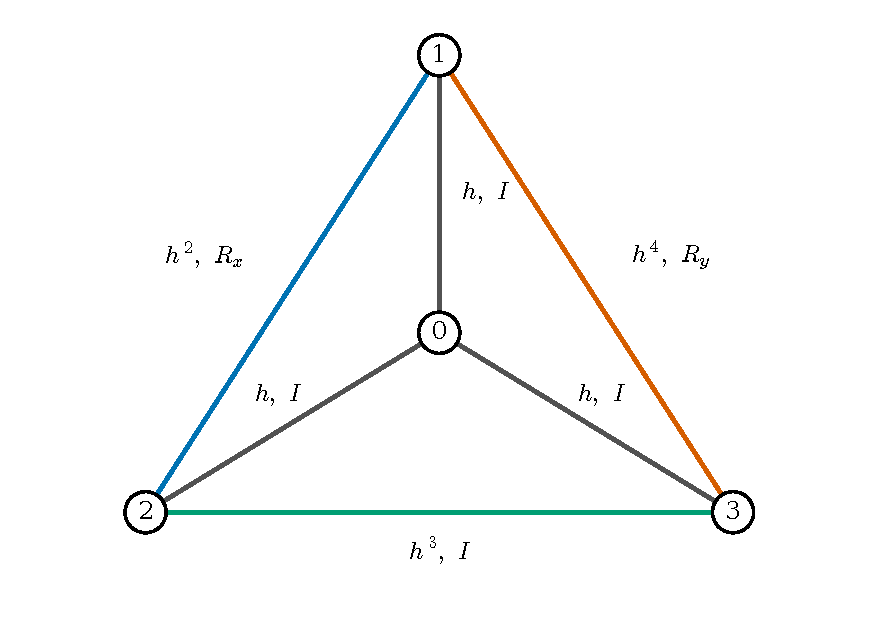
\includegraphics[width=.82\textwidth]{figures/output/three-scales.pdf}
 \caption{The actual attachment graph for the three-scale family.
 Each edge is labelled by its capacity weight and adjoint transport.
 The displayed transport on an edge $ij$, $i<j$, is from $j$ to $i$.
 The matrices $R_x,R_y$ are defined in \eqref{eq:rotations}.}
 \label{fig:three-scales}
\end{figure}

\begin{proposition}\label{prop:three-scales}
The twelve weak eigenvalues along this path satisfy
\begin{equation}\label{eq:three-scales}
 \begin{aligned}
 \lambda_0&\sim\tfrac12h^4,&
 \lambda_1,\lambda_2&\sim\tfrac12h^2,\\
 \lambda_3,\ldots,\lambda_8&\sim h,&
 \lambda_9,\lambda_{10},\lambda_{11}&\sim4h,
 \qquad \lambda_{12}\ge\gamma>0 .
 \end{aligned}
\end{equation}
Each member of a displayed group has the stated
asymptotic.
\end{proposition}
\begin{proof}
In three-by-three blocks the finite mass matrix is
$I_{12}$ and the energy matrix is
\begin{equation}\label{eq:three-scale-matrix}
 Q_h=\begin{pmatrix}
 3hI&-hI&-hI&-hI\\
 -hI&(h+h^2+h^4)I&-h^2R_x&-h^4R_y\\
 -hI&-h^2R_x^T&(h+h^2+h^3)I&-h^3I\\
 -hI&-h^4R_y^T&-h^3I&(h+h^3+h^4)I
 \end{pmatrix}.
\end{equation}
The order-$h$ star form has a three-dimensional kernel
$K=\{(x,x,x,x)\}$ and positive eigenvalues $1$ with
multiplicity six and $4$ with multiplicity three.
Thus nine eigenvalues have the asserted order-$h$
coefficients. The orthonormal embedding of $K$ is
$x\mapsto(x,x,x,x)/2$, and compression of the
order-$h^2$ coefficient is
\[
 \tfrac14(I-R_x)^T(I-R_x)
 =\operatorname{diag}(0,\tfrac12,\tfrac12).
\]
Trials in $K$ bound the remaining three eigenvalues
by $O(h^2)$. At such spectral parameters the
$K^\perp$ block is $hA+O(h^2)$ with $A>0$, and
its inverse is $O(h^{-1})$. The cross block is
$O(h^2)$, so its Schur contribution is $O(h^3)$.
Two eigenvalues are therefore asymptotic to $h^2/2$,
and one is $o(h^2)$.

The matrix is positive definite for $h>0$: zero
energy first forces a common vertex value, which
must be fixed by both $R_x$ and $R_y$; their fixed
axes meet only at zero. Direct expansion of the
printed matrix gives
\begin{equation}\label{eq:three-scale-det}
 \begin{split}
 \det Q_h=4h^{17}\big(&2+4h+14h^2+36h^3+55h^4+118h^5
                  +145h^6\\
                  &+194h^7+225h^8+178h^9+177h^{10}
                    +78h^{11}+54h^{12}\big).
 \end{split}
\end{equation}
The product of the nine fast eigenvalues is
asymptotic to $64h^9$, and that of the two middle
eigenvalues to $h^4/4$. Dividing the determinant by
these products gives $h^4/2$ for the remaining
eigenvalue. The relative comparison
\eqref{eq:relative-spectrum} transfers all these
coefficients to the actual operator.
\end{proof}

The accompanying exact calculation also verifies the
three rescaled characteristic-polynomial limits. For
$P(\lambda,h)=\det(\lambda I-Q_h)$ they are
\[
 \begin{aligned}
 h^{-12}P(hz,h)&\longrightarrow z^3(z-1)^6(z-4)^3,\\
 h^{-15}P(h^2z,h)&\longrightarrow-16z(2z-1)^2,\\
 h^{-17}P(h^4z,h)&\longrightarrow-8(2z-1).
 \end{aligned}
\]
These checks agree with the compression and determinant
argument above.

The inverse eigenvalue scales in
\eqref{eq:three-scales} are linearized relaxation
times. In particular, the weakest scale is not a
nonlinear tracking conclusion. In this example
$L_*=2\pi/h$ and $L_*\nu_0\sim\pi h^3\to0$,
so the all-time hypothesis in
Theorem~\ref{thm:all-time} below fails.
